\chapter{Design}
\label{design}
With promising results for machine learning based visual feedback a similar design could be made for Infandango.
\section{Language and Tools}
Two languages are immediate possibilities for implementation: Java\cite{java_site} and Python\cite{python_site}. I had most experience with Java, and some parts of Infandango were already written in Java. Most of Infandango was, however, written Python and I had some experience with it as well. After researching appropriate languages for machine learning R\cite{r_site} become a third possible choice. Follow research on all languages Python seemed most appropriate: integrating with Infandango would be straightforward and scikit-learn\cite{scikit_site} would remove the challenge of implementing machine learning methods.
\section{Proposed Design}
Using anonymised data from previous years a model can be built using machine learning methods. Using this model and some recent scores from the user, the following score can be predicted. There is however an unsolved problem here: How is the model trained?
\subsection{Model}
The Khan Academy model is built based on one assumption: a user can always \emph{generate another example} and it will be of the \emph{same type}. These are two qualities which Infandango does not share. Infandango has a preset number of manually written exercises and they are not grouped \emph{strictly} by similarity. The first proposed model was to take the average for each week and use those averages as features for the model. Then we must ask what is the model predicting? The only reasonable thing for it to predict would be the subsequent week's score. Although the simplicity is appealing there are some problems with this model. 

\begin{itemize}
\item If we are predicting the next week's score the problem turns into an estimating missing data problem, which is not a problem we want to solve
\item Even after 3-5 weeks there would only just be enough data to start getting reasonable results CITE HERE % CITE HERE graph, even though it is for later model
\item Grouping data like this means we have a lot less training examples
\end{itemize}

A similar alternative to this model is to treat each question within a week separately, giving the model a much larger dimensionality. Although this does remove the latter two problems, the first problem still remains. This adds the extra problem which is how to deal with situations where a student doesn't attempt a certain question.
\\
Both of these models have been working with the assumption that we want to learn something about \emph{specific} questions. So if, for example, a question was particularly hard then the model might be able to learn that it should predict lower scores for that question. However, we have seen that using specific questions as features causes other problems. For this reason a much simpler model was created. The model has \textit{\textbf{N}} features, each a percentage. Each feature represents a score from the corresponding previous question. The class is the score for the \textit{\textbf{N+1}} problem, so when a user is using the system it will try to predict their next score given their previous \textit{\textbf{N}} scores.

\subsubsection{Unexplored Alternatives}
% different kinds of features, moving average etc

\subsubsection{Retrieving Data}


\subsubsection{Machine Learning}
Django is used to query the database and get test results for all users. These test results are filtered into groups of \textit{\textbf{N+1}} consecutive results, with the final result being the class. For each set of \textit{\textbf{K}} results \textit{\textbf{K-N}} sets of results are created. This provides the machine learning methods with a lot more training data than alternative models.
\\%CAN ADD MORE HERE ABOUT TESTING OTHER RATIOS 
%can also talk about r2 scores
Using sci-kit learn's cross validation method the data was then split into training and testing sets, with a testing size of 20\%. Different machine learning methods were then trained on this data and tested by comparing their R2 scores. In Figure \ref{fig:comparison} it can also be seen that these tests are done multiple times over different values of \textit{\textbf{N}}. The highest accuracy is obtained by Logistic Regression at \textit{\textbf{N}} = 4. Logistic Regression is also the most consitent of the methods, making it an appropriate choice.

\begin{figure}[p]
\centering
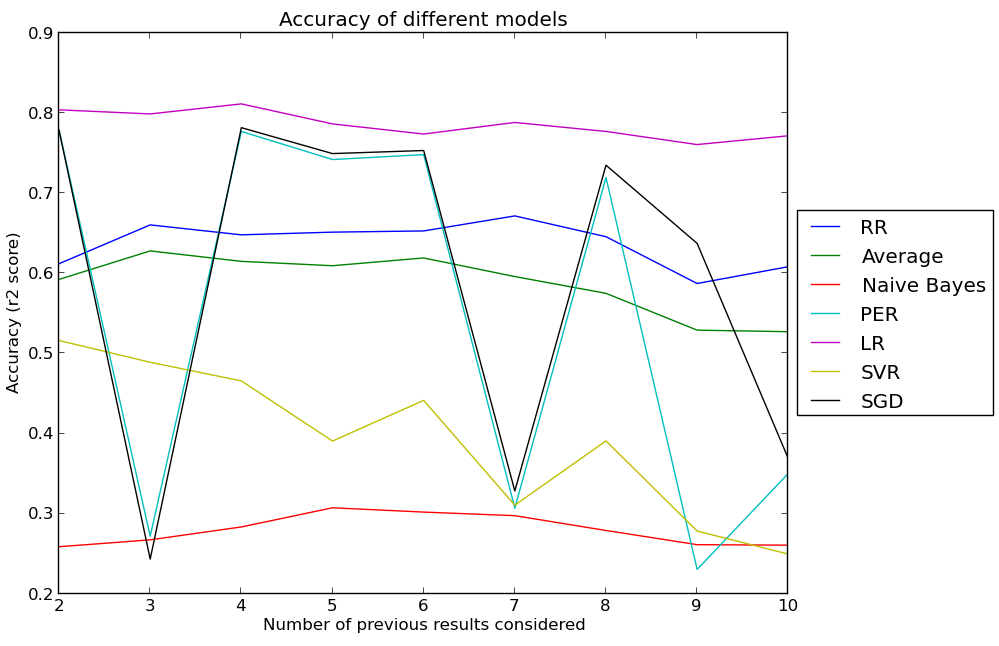
\includegraphics[width=1\textwidth]{comparison.png}
\caption{Comparison of different machine learning methods comparing their accuracy against the number of previous exercises considered}
\label{fig:comparison}
\end{figure}

%\subsubsection{Calibration}

\section{Integration with Infandango}
